% Supporting information for upgrade report

\documentclass[11pt]{article}
\usepackage{graphicx}
\usepackage[margin = 2.5cm]{geometry}
\usepackage[T1]{fontenc}
\usepackage{setspace}

% captions
\usepackage[labelfont=bf]{caption} %font=small,
\captionsetup{skip=7pt} 
\captionsetup{font=footnotesize,font={stretch=1.2}}

% tables
\usepackage{multirow}
%\usepackage{longtable} 
\usepackage{array}
%\usepackage{verbatim} 

%Line numbering
\usepackage{lineno}

% clinkable links 
\usepackage[hidelinks]{hyperref}
\hypersetup{
    colorlinks=false, %set true if you want colored links
    linktoc=all     %set to all if you want both sections and subsections linked
    %linkcolor=blue,  %choose some color if you want links to stand out
}

% line spacing
%\renewcommand{\baselinestretch}{2}



\begin{document}

\title{Supporting information for }
\author{Adrienne Etard}

\maketitle

% CONTENTS
\clearpage
\tableofcontents

%\cleardoublepage
%\addcontentsline{toc}{section}{List of Tables}

\clearpage
\listoftables
%\addcontentsline{toc}{section}{List of Figures}

\clearpage
\listoffigures

% \clearpage
% List of abbreviations

\clearpage

\section{Trait data compilation}

\subsection{Definition of diet categories}
% Diet trait and primary diet and trophic levels
For mammals and birds, diet was compiled from EltonTraits (ref). Primary diet was available in the avian dataset and declined in 5 categories: (1) plant or seed consumers; (2) fruit or nectar consumers; (3) 
For amphibians, diet information was extracted from AmphiBIO. 

\subsection{Habitat affinities and broad specialisation}
\paragraph{Habitat preferences.}
% Pooling in broader habitat categories
IUCN habitat data records habitat types in which species occur. Habitats are classified into 96 categories, which I pooled into 13 broader habitat variables: 
Forest, Savanna, Grassland, Shrubland, Wetland, Rocky areas, Caves and subterranean, Desert, Marine, Marine intertidal or coastal/supratidal, Artificial, Introduced vegetation and Other/Unknown. Species habitat preferences were described using these variables as binary (taking 1 if a species was known to occur in the habitat and 0 otherwise).
\paragraph{Habitat breadth.}
Habitat breadth was calculated as the number of habitats recorded to be used by a species in the IUCN database. Given that information regarding habitat suitability and habitat importance was also available in the IUCN data files, I used a weighted sum to calculate habitat breadth. Suitability was declined in three categories in the IUCN files: `suitable', `marginal' or  `unknown'. Habitats were recorded to be either of major importance, not of major importance or of unknown importance. I used the weights provided in Table \ref{weights} to produce weighted sums of the number of habitats used by each species. A comparison of the distribution of habitat breadths calculated with and without weights shows that weighting did not have a strong impact on the results (Figure \ref{distHB}).
\begin{table}[h!]
\renewcommand{\baselinestretch}{1}
\renewcommand{\arraystretch}{1.5}
\begin{center}\fontsize{9}{11}\selectfont
\caption[Weights used in the calculation of habitat breadth]{\textbf{Weights used in the calculation of habitat breadth.} Habitat breadth was calculated as the weighted sum of the number of habitats used by a species. Weights were assigned to each habitat given its importance and its suitability. All weights would equal 1 if habitat breadth was calculated as a non-weighted sum of habitat numbers.} 
\label{weights}
\begin{tabular}{|l|c|c|c|}
\hline
\multicolumn{1}{|c|}{\multirow{2}{*}{\textbf{Suitability}}} & \multicolumn{3}{c|}{\textbf{Major importance}} \\ \cline{2-4} 
\multicolumn{1}{|c|}{}                             & \textbf{Yes}       & \textbf{No}        & \textbf{Unknown}       \\ \hline
\textbf{Suitable}                                           & 1         & 0.5       & 1             \\ \hline
\textbf{Marginal}                                           & 0.3       & 0.3       & 0.3           \\ \hline
\textbf{Unknown}                                            & 1         & 0.3       & 1             \\ \hline
\end{tabular}
\end{center}
\end{table}

\begin{figure}[h!]
\centering
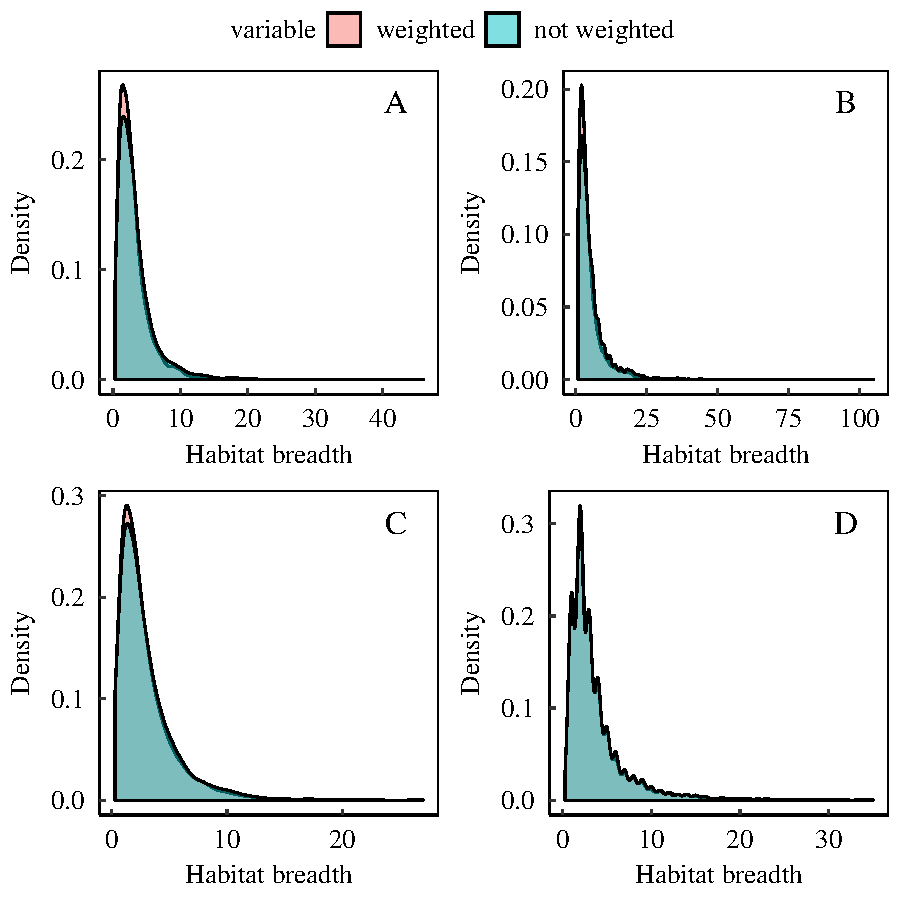
\includegraphics[scale=0.8]{figures/Weighted_HB/distributions}
\caption[Distribution of habitat breadths across species for terrestrial vertebrates]{\textbf{Distribution of habitat breadths across species for terrestrial vertebrates.}}
\label{distHB}
\end{figure}


\paragraph{Degree of specialisation.}
A broad classification was adopted for species degree of specialisation. Using IUCN habitat files, I determined whether species were strictly natural habitat specialists or generalists. Generalists were species for which any habitat, suitable or of unknown suitability, was recorded to be artificial. Else, species were considered to be natural habitat specialists. When a habitat of an unknown type was considered suitable or was of unknown suitability, missing data was introduced for the degree of specialisation. 



\subsection{Tackling taxonomic synonymy}
% Delta in species number before and after taxonomic corrections + typos.s

% Synonym table extract and number of manual additions.

% Replication in phylogenetic tips: case studies


\subsection{Imputation robustness}

\subsection{Trait distributions}



\end{document}